\documentclass{article}
\usepackage[a4paper, total={6in, 8in}]{geometry}
\usepackage[
backend=biber,
style=alphabetic,
sorting=ynt
]{biblatex}
\usepackage{graphicx}
\addbibresource{ref.bib}

\title{Space-based Laser Ablation for Debris Removal}
\author{Nikilesh Ramesh, Albie Gray, Bradley Bell, George Dixon, Jan Fraczek, Dongze Wu}
\date{February 2023}

\begin{document}


\begin{titlepage}
    \begin{center}
        \vspace*{1cm}

        \Huge
        \textbf{Space-based Laser Ablation for Debris Removal}

        \vspace{1.5cm}

        \Large
        \textbf{Nikilesh Ramesh, Albie Gray, Bradley Bell, George Dixon, Jan Fraczek and Dongze Wu}

        \vfill

        \large
        Technical Bid for Engineering You're Hired 2023
        \begin{figure}[htp]
            \centering
            
\includegraphics[width=6cm]{Images/EYH.png}
            \label{fig:EYH}
        \end{figure}

        The University of Sheffield \\
        February 2023
    \end{center}
\end{titlepage}
\tableofcontents
\newpage

\section{Problem Overview}

There are currently over 100 million pieces of junk in orbit around the planet, mostly objects smaller than 1cm \cite{EYHwebsite}. These objects pose a threat to operational satellites and future space missions as they travel at speeds up to 8 km per second \cite{ESA} and therefore have huge amounts of kinetic energy. The problem could spiral out of control if the debris begins to break up objects into smaller pieces, creating a chain reaction of destruction. Some challenges faced are the sheer number of objects needed to be moved or destroyed. Larger pieces of debris can be tracked and collisions avoided, but the smaller pieces are much harder to track and thus have created problems caused by high speed collisions. Our efforts to remove the debris must not create any junk in the process, be it during launch or operation and we must not pose a threat to the people on earth by any falling debris.  We have to act fast to reduce the amount of debris in orbit or face detrimental consequences in the future.
\section{Technical Details}
\subsection{Proposal}
The proposed solution for space debris removal is a space-based laser ablation. This solution particularly focuses on the removal of small and irregularly shaped debris in the Low Earth Orbit. This class of debris poses a major threat to the various science, communication and other types of satellites that use this orbit. 

A satellite or a network of satellites weighing approximately 1 ton equipped with a precise laser system capable of delivering an energy pulse of 600J \cite{SBL} can be used to de-orbit the small debris. Every energy pulse delivers kinetic energy, ideally in the opposing direction, this decreases the total kinetic energy of the debris which subsequently leads to the drop in velocity. 
    \begin{figure}[htp]
            \centering
            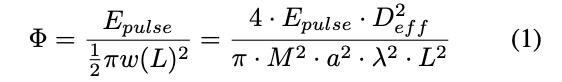
\includegraphics[width=6cm]{Images/EDen.png}
            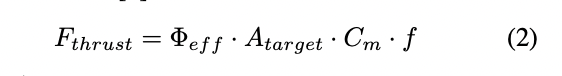
\includegraphics[width=6cm]{Images/Thrust.png}
            \label{fig:EYH}
        \end{figure}

Over multiple interactions, the velocity of the debris is slowed to below the critical orbital velocity, thus leading to re-entry.

        \begin{figure}[htp]
            \centering
            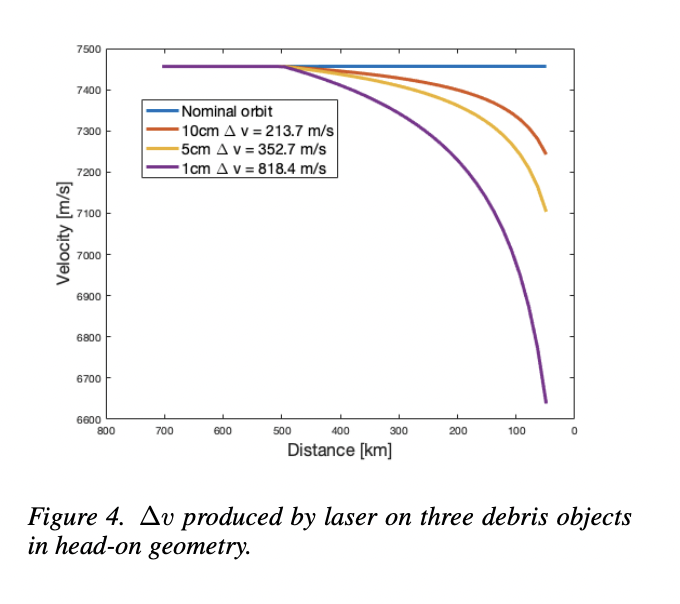
\includegraphics[width=6cm]{Images/NominalOrbit.png}
            \label{fig:EYH}
        \end{figure}
        
\subsection{Technical Challenges}
This approach works best when the satellite meets the debris in an head-on geometry and are co-planar. It works with other combinations of geometry but with reduced efficiency, many more interactions will be required to de-orbit. One solution to this is using a network of satellites to cover a large possible combinations of geometry.

Precise and accurate tracking is another technical challenge, institutions like NASA already have a network of satellites to track debris, the proposed satellites can also join this network to collect and share data on the debris. This would require the satellites with high-tech sensors which put strain on the budget and complexity of the mission.
\subsection{Cost}
Companies like AST SpaceMobile, Black Sky and Eutelsat manufacture satellites costing between 10 and 60 million dollars. The Starlink satellite produced by SpaceX costs between 250 to 500 thousand dollars to make. This is a more realistic valuation for our satellite as it is of similar dimensions as well as it operates at a similar orbital height to our design. The cost of the laser the satellite will be fitted with is hard to judge but looking at lasers with a similar power output it is likely to be around a million dollars. Assuming we use the SpaceX service to put our satellite into orbit, the cost per unit is anywhere between 2.5 and 3 million dollars. To estimate the final cost of the entire mission including Research and Development, a R\&D to product ratio was used \cite{RD}, which puts the mission cost at around 12 million spread out over an estimated 10 year mission timeline.

\subsection{Product Lifecycle}
The product is expected to have a similar life cycle to that of an average satellite which is approximately 15 years. The end of a satellite’s lifecycle is usually marked by the exhaustion of the propellant aboard. The one significant difference when it comes to this design is that the satellite is set to de-orbit itself and burn up in earth’s atmosphere before it reaches the end of its fuel reserve.


\subsection{Project Management}
This project has an estimated timeline of 10 years. A Gantt Chart has been produced with the high-level tasks that will be completed. These tasks can be further broken down into sub-tasks by the team in order to ensure that the solution is achievable.

\subsection{Risk Assessment and Safety}
As with every space mission there are big risks associated with it. Some safety issues arise while launching the satellite like it crashing before it makes orbit as well as crashing while in orbit. The other obvious safety issue is associated with the laser, these might include it targeting the wrong object or causing debris to change course in a wrong way and cause damage to other satellites. There is also the legal side of things, the laser can only be used for the purpose of destroying debris, some might view it as a weapon. Further research has to be done on the impact of the laser on the ozone layer and the environment.

\subsection{Patent or intellectual property/licensing information}
A patent is an exclusive right granted for an invention, which is a product or a process that provides, in general, a new way of doing something, or offers a technical solution to a problem \cite{WIPO}.

Once the satellites are in operation, a patent can be applied for regarding the laser aspect, which is the USP of this product. This can be to ensure that no other companies are able to copy, thus achieving longevity and sustainability. 
Earth-to-space lasers are already operational, however in-space lasers are not and the idea is an innovative design - applying for a patent for this would therefore be reasonable.

\section{Cybersecurity Statement}
Cybersecurity is critical to this organisation. It is imperative that access to systems is continuous, intellectual property is protected and personal data is protected. It must also be ensured that legislation such as the Data Protection Act and the General Data Protection Regulation (2018) are followed closely \cite{GOV}.

\subsection{Company Responsibilities}
\begin{itemize}
    \item Employees will have regular training on recognising different types of social engineering
    \item Links from external sources will be blocked
    \item There will be a dedicated IT specialist who can assist employees in identifying malicious material
    \item Antivirus software will be updated regularly
    \item Multi-factor authentication will be used
    \item DDos protection will be provided by companies such as cloudflare and imperva 
\end{itemize}

\subsection{Individual Responsibilities}
\begin{itemize}
    \item Passwords should be secure and unique for this system
    \item Passwords should never be written down or shared with anyone
    \item When working remotely, no sensitive information should be viewed on unsecured networks
    \item Use of a VPN and Antivirus are mandatory and must be kept updated
    \item Devices should never be left unattended
\end{itemize}

\section{Sustainability}
Sustainability is an integral part of any idea proposal, ours being no exception. It is crucial that our solution maintains a high standard of sustainability throughout each stage - from the initial design idea to the end-of-life of the product.
\subsection{Detrimental Impacts}
It is important that our proposed idea holds no impacts that may cause more harm than good. This greatly affects sustainability because, effectively, it means that the solution is not a good one and needs to be disregarded. 
Impacts such as:
\begin{itemize}
    \item Causing more space debris.
    \item Causing more risks to bodies in space, human or otherwise
    \item Ineffective clear-up of ‘space junk’
\end{itemize}

\subsection{Ethical Considerations}
A product is deemed unsustainable if it wasn't made in a socially responsible way (in a poor working environment). 
Therefore, it is imperative that health and safety regulations are set up in the early stages to clearly outline the workers rights and what they are/are not entitled to. If this is done correctly, the project can be considered "socially sustainable". Some examples \cite{TUC} are:
\begin{itemize}
    \item A break after an allotted amount of time.
    \item Legitimate safety equipment when working with dangerous machines.
    \item Adequate lighting, heating and ventilation for worker comfort.
    \item Staff facilities (including toilets)
\end{itemize}

\subsection{Economic Factors}
It is exceedingly difficult, especially during aerospace applications, to keep the cost of the product low. This is due to the nature of the application: being able to launch bodies into space, along with selecting the materials that can withstand escaping the atmosphere into orbit, is expensive. 
However, as long as at every stage the cheapest option is sought after while ensuring it still holds the highest performance capability, the product is a success.

\section{Team Profile}
\subsection{Bradley Bell}
Aerospace Engineering
Responsibilities: Responsible for looking into statistics in order to focus on issues, funding as well as methods of laser ablation.


\subsection{George Dixon}
Mechanical Engineering
Responsibilities: Responsible for researching methods for launch, the cost implications of this and also deorbiting techniques.




\subsection{Jan Fraczek}
Civil and Structural Engineering
Responsibilities:: project choice matrix, cost evaluation, risk analysis as well as presenting on different aspects of the project.


\subsection{Albie Gray}
Computer Science
Responsibilities: Researched the funding, sustainability, and wrote the cybersecurity statement. Presented throughout the project.


\subsection{Nikilesh Ramesh}
Aerospace Engineering
Responsibilities: Responsible for technical information collection, project management projections as in Gantt charts and presenting the information to the EYH board.

\subsection{Dongze Wu}
Material Science
Responsibilities: Worked on manufacturing and presented on various aspects of the project.

\printbibliography
\end{document}
